 \section{Improved prototype}
\label{interface}

The new interface contains usability updates, such as information tooltips, custom input fields and a start screen with a limited set of predetermined \emph{core} constants.
%hover-over tooltips to explain the meaning of the constants and custom input fields for numerical domains. The user is also initially presented with a small set of predetermined \emph{core} constants, and can expand this set to \emph{relevant} constants 
%\footnote{See further in Section~\ref{interface} for more information on relevance.}
%or simply \emph{all} constants.
%: initially, only constants with the highest priority are shown and the user must expand the view to see also constants of a lower priority. 
A more important improvement is the clear distinction between  \emph{chosen atoms} (set by the user) and  \emph{propagated atoms} (implied by the chosen atoms).
The interface visualizes chosen atoms by a $\circlearrowleft$-symbol to indicate that this choice can be reconsidered. Propagated atoms are visualized by question marks, indicating that they can be \emph{explained}.
%\paragraph{First interactive decision enactment interface}
%In legislation the use of a large number of concepts that are defined at a very fine-grained level are common.
%Often, the definition themselves contain concepts that need to be defined.
%From an end-user point of view this creates a challenge to keep the interface clear.
%The interface proposed in \cite{Ingmar} does not make a distinction between important, often used concepts and less used concepts.
%All of the available concepts are shown in one screen, which is a disadvantage given the large number of fine-grained concepts.
\begin{comment}
As before, the interface operates independently of the domain knowledge gathered in the knowledge base.
This is still the case in the new interface.
Additionally, a separate \emph{comma separated value} file -- denoted as \emph{the CSV} -- is required as input.
The CSV contains some configuration options and meta-information on the symbols to be used by the \ides.
A first piece of meta-information is a priority value for symbols and atoms. This priority value determines which concepts are shown first to a user.
%Initially, only atoms with priority code $1$ are displayed, while atoms with priority code $2$ are displayed when the view is expanded.
Other pieces of meta-information are information strings for symbols and atoms, which allow the \ides~to elaborate on the intended meaning of symbols and atoms in the knowledge domain.
In this application we used it to reference the applicable law article.
\end{comment}
%Also, these information strings are convenient for explaining concepts that are used in the knowledge domain, but are not really part of it.
%E.g., special rates exist for the purchase of monuments (subject to conditions).
%In our current model, we expect the user to know whether or not the real estate can be classified as a monument, so we treat this as a simple Boolean input.
%However, the criteria for buildings to be monuments are determined in a separate decree, and an information string can refer to this decree.
%To avoid confusion and enable use for less versed users, these fine-grained definitions needed to be modelled in the previous interface, leading to excess literals and code.
%In the new interface, more abstract definitions with textual explanation suffice.
%The user can request these strings by hovering over or clicking on a dedicated information button
%The result is a more focused and concise domain knowledge base.
%Further improvements to the \ides~ comes from the new inferences of \textit{relevance} and \textit{explanation}, that are discussed in the following sections.
The most significant improvement is the application of the  \textit{relevance} and \textit{explanation} inferences for interactive decision enactment. 
%Both are refinements of algorithms that already existed in \idp, but that had not yet been used in the context of interactive decision enactment. 

\paragraph{Explanation} to increase user confidence, it is important that the system is able to explain why it derived certain conclusions. 
%At times the use of the \ides~ may lead to unanticipated or even unwanted outcomes, where a user did not expect a propagated atom to be set to true or false.
Moreover, the user sometimes would like to flip a propagated atom's truth assignment.
%In this situation, it is crucial that the propagated atom assignments are explained to clients.
%The identification of chosen atom assignments allows the user to revise his choices and perhaps change the outcome of his query.
%
The explanation inference identifies the chosen atoms that imply a propagated atom, and allows to revise these choices.
%\jo{I refined the inference, but at its core, the inference was already implemented in \idp. Should we mention any of this?}
%\Marjolein{we already mention something similar for the relevance inference. maybe we extend the remark to explanation, rather than repeating it here? --- hm, ik dacht dat dit ergens algemeen vermeld was, maar ik zie  nu dat het bij relevance staat. dan kan je het moeilijk algemener maken natuurlijk.  Als er al over gepubliceerd is, kan je er best ook naar verwijzen, niet?}
As input, it takes a theory $T$, a partial interpretation $\ci$ and a propagated atom $a$. %Propagated assignments (i.e., those that were not chosen by the user but derived by the \emph{propagation} inference) are 
%a shared vocabulary, as well as a single atom assignment $a \mapsto v$ (with $v \in \{\true,\false\}$) propagated from $T$ and $I$.
%More formally, $I \cup \{a \mapsto \neg v\} \not \models T$, or $I$ extended with $a \mapsto \neg v$ can not be expanded to a model for $T$.
As output, it returns a least precise partial interpretation $\ci^{expl}$ such that $a$ would still be propagated by $\ci^{expl}$.
%minimal set of atom assignments $A$ from $I$ such that for structure $I'$ formed by merging $A$ with $I$'s type interpretations, it holds that $I' \cup \{a \mapsto \neg v\} \not \models T$.
%In words, the explanation inference calculates a minimal substructure $I'$ of $I$ that still propagates $a \mapsto v$ under $T$.
\begin{figure}[]
	%\centering	
	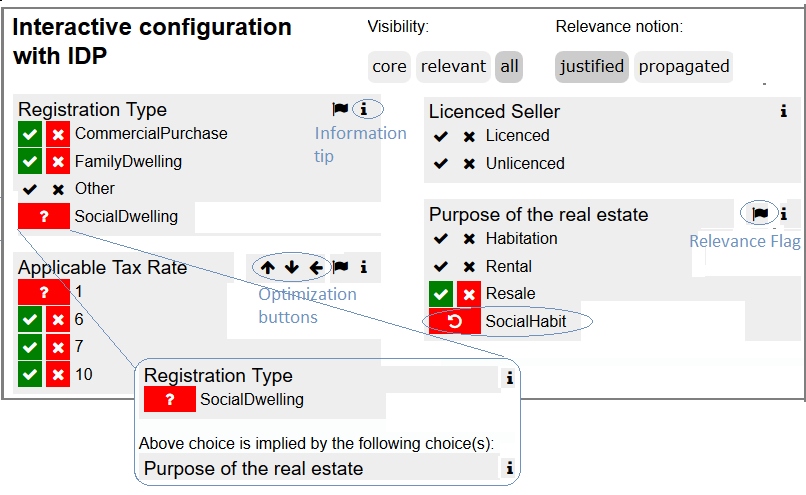
\includegraphics[angle=0,width = 1 \columnwidth]{img/26102018quat.png} %, trim={2.5cm 21,7cm 2,2cm 2,0cm}, clip]
	\caption{Relevance and explanation demonstrated in the new interface.}
	\label{fig:relevance}
\end{figure}
This is demonstrated in Figure~\ref{fig:relevance}.
When a user clicks on the question mark of a propagated atom $a$, the system constructs the partial interpretation $\ci_{chosen}$ from all the chosen atoms, and feeds $a$ and $\ci_{chosen}$ to \idp's explanation inference together with the theory $T$ containing all domain knowledge. The output then represents a minimal subset of all chosen atoms that still imply $a$'s propagated value, which is presented to the user as an explanation for the propagation.
%An overlay pops up, summarizing the minimal set of user choice atoms leading to the propagated atom.
%As shown in Figure~\ref{fig:relevance}, the user can consult the related law article directly by using the information button in the explanation box.

\begin{comment}
\Marjolein{Figure \ref{fig:interface} shows an edited screenshot of this process. The user has requestfed an explanation for the atom $RegistrationType=familyDwelling \mapsto \true$.
The overlay contains the user inputted atoms $TypeOfPurchase=naturalPerson \mapsto true$ and $PurchasePrice=210$, but does not include the user choice of $TypeOfPurchaser=naturalPerson \mapsto \true$, which is not part of an explanation for $RegistrationType=familyDwelling \mapsto \true$.}
\Marjolein{te vervangen door onderstaand stuk}


%\jo{Todo: figuur toont 2 explanations, tekst vertelt over 1.}
%\Marjolein{zal eerst je tekst een nalezen dan :-)}

\begin{example}
\label{ex:explanation}
Starting from example \ref{ex:voctheostruct} we extend theory $T_{ex}$ in which the ApplicableRate is defined with the following definitions of registration type, the allowed selling price limit for family dwellings and a trivial constraint:
\begin{align*}
&\{ HasRegistrationType = socialDwelling \leftarrow Seller = licensedSeller \\
& \indent \wedge Purpose = socialHabitation. \\
& HasRegistrationType = familyDwelling \leftarrow BuyerType = naturalPerson \\
& \indent \wedge Price \leq Limit. \\
& HasRegistrationType = other \leftarrow HasRegistrationType \neq socialDwelling \\
& \indent \wedge HasRegistrationType \neq familyDwelling.\} \\
& \exists x \colon HasRegistrationType = x.\\
&\{Limit = 220 <- Municipality = Antwerp \vee Municipality = Brussels.\\
&Limit = 200 <- Municipality = otherMunicipality.\}
\end{align*}
Input structure $I_{ex}$ is expanded with:
 \begin{align*}
 & BuyerType^I = \{naturalPerson\}\\
 & Price^I = \{220\}\\
 & Municipality^I = \{Antwerp\}
 \end{align*}

% results in the following atoms after propagation
%As the result of the propagation of structure $I_{ex}$ over $T_{ex}$  $a \mapsto v$ with $v\in \{\true\}$:
The propagation of structure $I_{ex}$ over $T_{ex}$ rsults in the following atoms:
 \begin{align*}
     atoms^I = \{
& HasRegistrationType=familyDwelling \mapsto \true, \\
& ApplicableRate=7 \mapsto \true, \\
& BuyerType=naturalPerson \mapsto \true,\\
& Municipality=Antwerp \mapsto \true,\\
& Price=210 \mapsto \true,\\
& Limit=220 \mapsto \true,\\
& HasRegistrationType=other \mapsto \false,\\
& HasRegistrationType=socialDwelling \mapsto \false,\\
& ApplicableRate=1 \mapsto \false,\\
& ApplicableRate=10 \mapsto \false,\\
& Limit=200 \mapsto \false \}
\end{align*}
If the user requests an explanation for the atom ApplicableRate=7 $\mapsto \true$, the inference \textit{explanation} searches for the minimal set of atoms in $I_{in}$ that explain the interpretations in $I_{out}$.  For this example the $ApplicableRate$ is determined by the $BuyerType$, $Municipality$ and $Price$, as shown in figure \ref{fig:interface}.
\end{example}
\begin{figure}[h]
	\centering	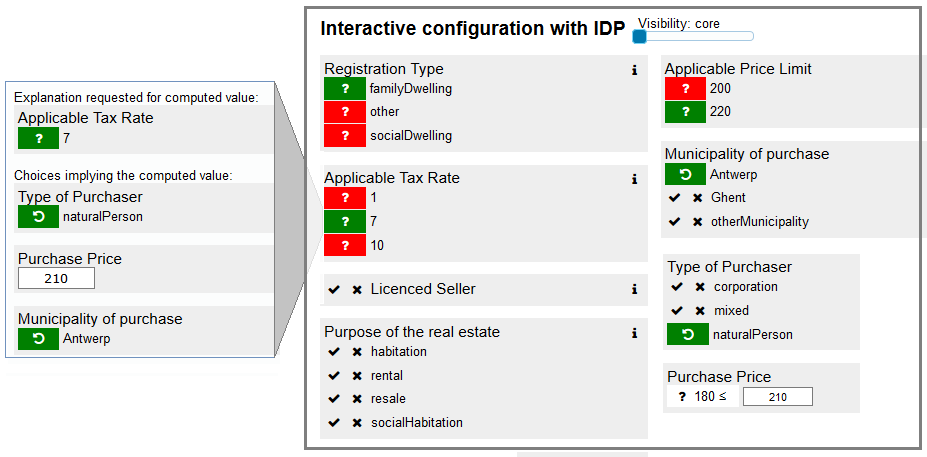
\includegraphics[angle=0,width = 1
	\linewidth]{img/explanation.png} %, trim={2.5cm 21,7cm 2,2cm 2,0cm}, clip]
	\caption{Propagation and explanation in the new \ides.}
	\label{fig:interface}
\end{figure}
\end{comment}
 
\paragraph{Relevance}
\label{sec:relevance}
A key problem of the original prototype was that it encouraged notaries to ask irrelevant questions. For instance, the knowledge base included the concept of a \emph{licensed seller}: only when the seller is licensed, can the property be eligible for a social registration. In particular, the definition of $RegistrationType$ contains the following rule:
\[\left\{\begin{aligned}
 & RegistrationType = Social \leftarrow \\ 
 & Seller=Licensed~\land~Purpose=SocialHabit.
\end{aligned}\right\}\]
Moreover, this is the only formula where the licensed seller concept is used. Once the notary has determined that the purpose of the real estate is not social habitation, there is no longer any need to determine whether the seller is licensed. %However, the original prototype would keep on displaying this as an undecided atom, tempting the notary into inquiring about it.

%In Section \ref{original}, some of the difficulties and solutions to design a clear interface given the inherent complexity of legislation, were discussed.
%In this section we discuss the \emph{relevance} inference as an important aid to keep track of necessary parts of information.
%Also, the relevance inference allows the system to signal the user that a current configuration of incomplete atom assignments suffices to satisfy all constraints in the problem domain, avoiding choices on irrelevant atoms.

%Informally, relevance inference pinpoints all unassigned atoms that can still contribute to satisfying a not yet satisfied constraint. Conversely, all unassigned atoms that have no possible impact on the truth value of any constraint are considered irrelevant.

Our new prototype makes use of the relevance inference to avoid this problem. This inference takes as input a theory $T$, a partial interpretation $\ci$ that is closed under propagation, and a set of \emph{goal constants} $C$. 
Its output is a set of \emph{relevant} atoms $a=v$ that can still affect the interpretation of the constants in $C$, given $T$ and the information present in $\ci$. 
In our example, if $\ci$ is such that $SocialHabit \in Purpose^\ci$ and $C = \{RegistrationType\}$, then the atom $Seller = Licensed$ is relevant, as choosing its truth value determines whether $RegistrationType=Social$.
If $SocialHabit \not\in Purpose^\ci$, then $RegistrationType=Social$ is false in all model expansions of $\ci$ w.r.t.~$T$, and $Seller = Licensed$ is therefore not relevant.
%The constants in $C$ will be called the \emph{goal constants}.

\idp's relevance inference is 
%a refinement of methods that were initially developed in order to improve \idp{}'s internal search routines~\cite{ijcai/JansenBDJD16}. %, but the registration duty use case motivated the development of a full-fledged relevance inference.
%The notion of relevance 
%It is 
based on justification theory (e.g., \cite{lpnmr/DeneckerBS15}). 
% As mentioned in Section~\ref{KBP}, the language that we use in this paper is a highly simplified version of the real \fodot language used in \idp. 
The concepts we introduce in the following paragraphs are highly simplified versions of the original justification theory and of the implementation of the relevance inference that is available in our software tool. %, of which we describe a simplified version here.

%\jo{The following is too detailed for a 4-page paper. I would prefer a reference to Joachim's relevance paper instead.}
The \emph{dependency graph} of a theory $T$ has all of the subformulas of the theory as its nodes and has an edge from each formula to all of its subformulas. In addition, for each rule of the form $A \leftarrow \varphi$, there is also an edge from the atom $A$ to the formula $\varphi$. Intuitively, each directed edge from $\varphi$ to $\psi$ in this graph means that the truth of $\varphi$ is defined (or can be \emph{justified}) by the truth of $\varphi$. Finally, we also add each of the goal constants $C$ to the graph and include an edge from each goal constant $c \in C$ to all atoms of the form $c=v$. The idea behind these edges is that value of the goal constant $c$ is influenced by the truth of these atoms $c=v$. We denote the resulting graph by $G^C_T$.
\begin{comment}
Figure \ref{fig:dependency} demonstrates the dependency graph for our limited example in which the applicable rate is determined by the registration type.



\begin{figure*}[]
	\centering	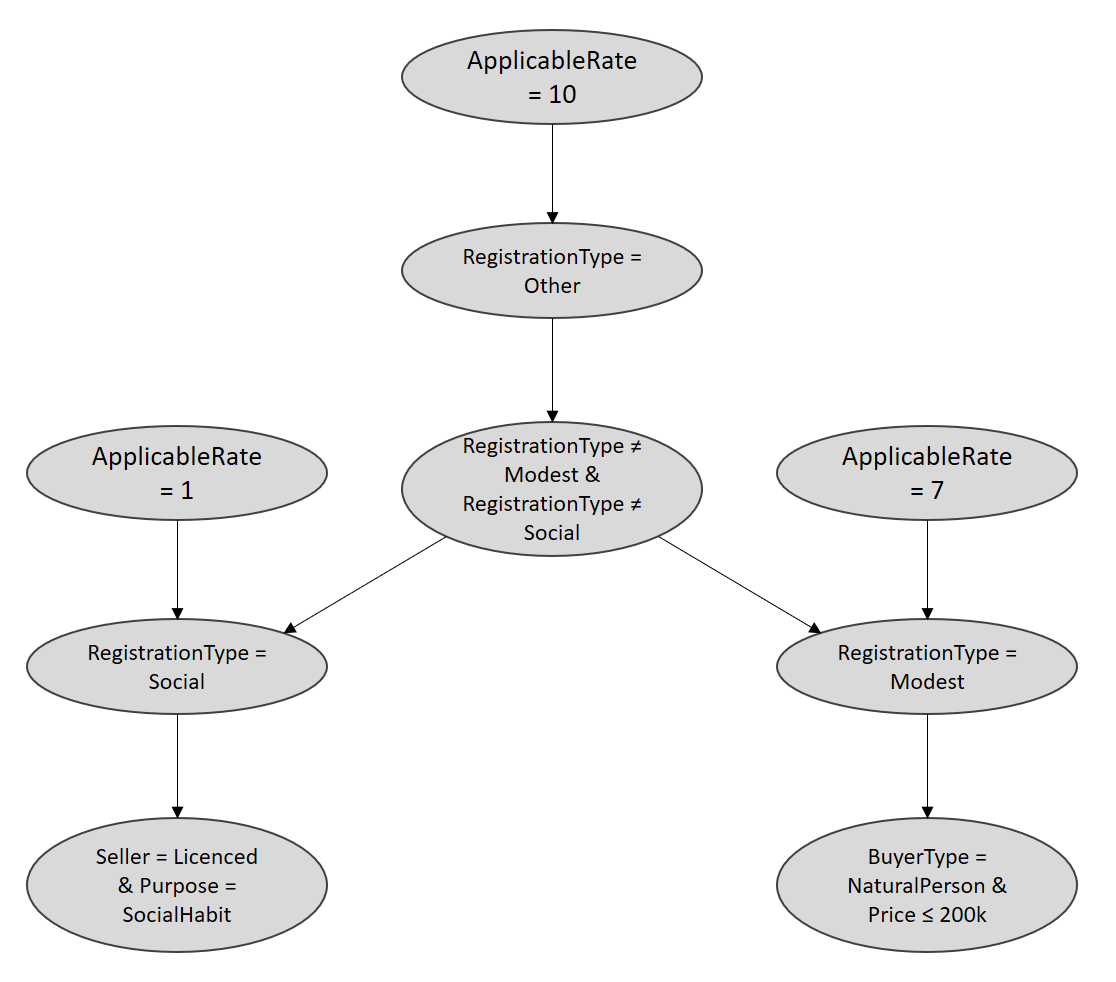
\includegraphics[angle=0,width = 0.6
	\linewidth]{img/dependency.png} %, trim={2.5cm 21,7cm 2,2cm 2,0cm}, clip]
	\caption{Dependency graph for the example theory.}
	\label{fig:dependency}
\end{figure*}
\end{comment}
%The sinks of $G^C_T$ are all atoms that do not appear in the head (i.e., at the left of the $\leftarrow$ symbol) of any rule in $T$. We call these sinks the \emph{open atoms} $Open(G^C_T)$ of the graph; intuitively, their truth value does not depend on that of any other node in the graph. By $\ci\lvert_{Open(G^C_T)}$ we denote the least precise partial interpretation $\ci'$ that such that, for each atom $c=v$ in $Open(G^C_T)$, $c^\ci = c^{\ci'}$. 
We say that a formula $\varphi$ is $T$-\emph{determined} by $\ci$ if either $\ci \models_T \varphi$ or $\ci \models_T \lnot \varphi$. Finally, we define that an atom $c=v$ is \emph{relevant} if it is not $T$-determined by $\ci$ and there exists a path in $G^C_T$ from this atom to one of the goal atoms, which does not traverse any node that is $T$-determined by $\ci$. %$\ci\lvert_{Open(G^C_T)}$.
%Intuitively, an atom is relevant if its truth value may affect the value assigned to one of the goal atoms \emph{and} this possible effect is not blocked by the fact that the truth value of some intermediate formula is already fixed by the current partial interpretation. In case of the above example, $Purpose \neq SocialHabit$ would $T$-imply $RegistrationType \neq Social$ and therefore making this choice would make $RegistrationType = Social$ $T$-determined. Hence, $RegistrationType = Social$ blocks the path from $Seller = Licensed$ to the goal constant $RegistrationType$, making this atom irrelevant. 

%This basic notion of relevance can be further refined in order to better handle special cases such as unfounded choices and recursive definitions~\cite{ijcai/JansenBDJD16}, but this is out of scope of this paper.

%To define what relevant atoms are, we need the notion of a \emph{dependency graph} of a theory.
%A theory's dependency graph has a theory's formulas as nodes, and has a directed edge from a formula to its subformulas, or from a formula in the head of a rule to the formula acting as the body of a rule.\jo{citation needed}
%By a process called \emph{grounding} using a structure's type interpretations, the dependency graph can be simplified such that each node is a unique atomic formula -- an atom.
%Atoms that have no outgoing edges in the dependency graph are called \emph{open}, atoms that have no ingoing edges are \emph{root}.
%In the registration duty use case, the dependency graph is acyclic, thus it forms a tree. \jo{is this "tree-ness" needed?}

%\begin{definition}
%Let $G_T$ be a dependency graph of a theory $T$ with only atom nodes, and let $I$ be a structure over $T$'s vocabulary which is closed under propagation with $T$ and which can be expanded to a model for $T$.
%An atom $a$ is \emph{justified} if $a \mapsto v$ with $v \in \{\true,\false\}$ is in $I$, if there exists a substructure $open(I)$ of $I$ where all true or false atoms are open in $G_T$, and where $open(I) \cup \{a \mapsto v\} \not \models T$ for some $v \in \{\true,\false\}$.
%\end{definition}
%Informally, an atom is justified if its truth value is fixed by an assignment to open atoms.

%\begin{definition}
%Let $G_T$ be a dependency graph of a theory $T$ with only atom nodes, and let $I$ be a structure over $T$'s vocabulary which is closed under propagation and which can be expanded to a model for $T$.
%An atom $a$ is \emph{relevant} if it is not justified by $G_T$ and $I$, and if it is reachable in $G_T$ from an unjustified root atom by only traversing unjustified atoms.
%\end{definition}
%Informally, root atoms in a dependency graph represent constraints in $T$, and relevant atoms are those that might still justify an unjustified constraint.

%Now, the relevance inference takes as input a theory $T$ and structure $I$ over a shared vocabulary, such that $I$ is closed under propagation with $T$ and $I$ can still be expanded to a model of $T$, while its output is simply the set of atoms relevant under $T$ and $I$.

%\begin{example}
%\label{ex:relevance}
%\Marjolein{code verplaatst naar explanation : Consider the following theory which defines the registration type and has a trivial constraint:
%\begin{align*}
%\{ & HasRegistrationType = socialDwelling \leftarrow Seller = licensedSeller \\
%& \indent \wedge Purpose = socialHabitation. \\
%& HasRegistrationType = familyDwelling \leftarrow BuyerType = naturalPerson \\
%& \indent \wedge Price \leq Limit. \\
%& HasRegistrationType = other \leftarrow HasRegistrationType \neq socialDwelling \\
%& \indent \wedge HasRegistrationType \neq familyDwelling.\} \\
%& \exists x \colon HasRegistrationType = x.
%\end{align*}

%In case the estate has not been destined for social habitation, we can construct a structure $I$ with only assigned atoms $Purpose = socialHabitation \mapsto \false$ (the estate's purpose can not be social habitation) and the implied $HasRegistrationType=socialDwelling \mapsto false$ (the registration type can not be a social dwelling).}
%Consider the theory from example \ref{ex:explanation} and an  interpretation $I_{rel}$ that contains the assigned value for $Purpose$ and the propagated value for $socialDwelling$:
%\begin{align*}
%    &Purpose = socialHabitation \mapsto \false\\
%    &HasRegistrationType=socialDwelling \mapsto \false
%\end{align*}

%$I$ is closed under propagation with $T$, but there still exists an expansion of $I$ to a model of $T$.
%Now, the output of the relevance inference with $T$ and $I$ as input will not contain the atom $Seller=licensedSeller$, as it could only be reached from the constraint $\exists x \colon HasRegistrationType = x$ through the node $HasRegistrationType = socialDwelling$, which is justified as $Purpose = socialHabitation\mapsto false$ is an open, assigned value in $T$'s dependency graph.
%In other words, whether the seller of the estate is a licensed seller, is not relevant, and it is not needed to fix the value of the corresponding atom.

%Similarly, if the registration type is not a social dwelling or a family dwelling, the registration type must be ``other'', satisfying the unique constraint, and making any further unassigned atoms irrelevant.
%%in praktijk na te kijken of dit ook zo in de interface aangegeven wordt!
% iets toe te voegen over constraint
%\Marjolein{ik zou de laatste zin weglaten: het principe wordt reeds duidelijk uitgelegd voor licencedSeller}
%\end{example}

In the interface, a relevant choice $c=v$ is highlighted with red and green buttons (to assign it true or false), while irrelevant choices can still be made, but the buttons are grey. In addition, the box for a constant $c$ is flagged in the upper right corner to indicate that at least one relevant atom over $c$ still exists. Finally, it is also possible to hide irrelevant unknown atoms. %The choices of the relevant atoms themselves are highlighted in green and red.
Figure \ref{fig:relevance} shows the atom $Seller=Licensed$ is indeed irrelevant (for the implicit goal constant $RegistrationType$) under the given truth assignment.



